\documentclass[xcolor=dvipsnames]{beamer}
\usepackage[T1]{fontenc}
\usepackage[utf8]{inputenc}
\usepackage[english,slovak]{babel}

\usepackage{amsmath}
\usepackage{amsthm}
\usetheme{Pittsburgh}
\useoutertheme{shadow}

\usepackage{graphicx}
\usepackage{caption}
\usepackage{subcaption}

\usepackage[]{algorithm2e}
\usepackage{listings}
 \setbeamercovered{transparent}
 \usepackage{cuted}
\usepackage[export]{adjustbox}
\usepackage{mathtools}

\usepackage{lipsum}
\usepackage{verbatim}
\usepackage{transparent}
\usepackage{framed}
\usepackage{xcolor}

\usepackage{multirow}
\usepackage{colortbl}
\usepackage{lmodern}

\usepackage{movie15}
\usepackage{media9}
\usepackage{verbatim}

\usepackage{animate}


\usepackage{hyperref}

\newcommand\Wider[2][3em]{%
\makebox[\linewidth][c]{%
  \begin{minipage}{\dimexpr\textwidth+#1\relax}
  \raggedright#2
  \end{minipage}%
  }%
}






\iftrue

\usetheme{Warsaw}

\setbeamercolor{normal text}{fg=white,bg=black!90}
\setbeamercolor{structure}{fg=white}

\setbeamercolor{alerted text}{fg=red!85!black}

\setbeamercolor{item projected}{use=item,fg=black,bg=item.fg!35}

\setbeamercolor*{palette primary}{use=structure,fg=structure.fg}
\setbeamercolor*{palette secondary}{use=structure,fg=structure.fg!95!black}
\setbeamercolor*{palette tertiary}{use=structure,fg=structure.fg!90!black}
\setbeamercolor*{palette quaternary}{use=structure,fg=structure.fg!95!black,bg=black!80}

\setbeamercolor*{framesubtitle}{fg=white}

\setbeamercolor*{block title}{parent=structure,bg=black!60}
\setbeamercolor*{block body}{fg=black,bg=black!10}
\setbeamercolor*{block title alerted}{parent=alerted text,bg=black!15}
\setbeamercolor*{block title example}{parent=example text,bg=black!15}

\fi



%-------------------------------------------------------------------------------------
\title{\color{white} \bf deep reinforcement learning 1 - DQN and DDPG}
\author{\color{white} Michal CHOVANEC, PhD}


%\setbeamertemplate{footline}[frame number]{}
\setbeamertemplate{navigation symbols}{}


\date[EURP]{}
\begin{document}

{
    \usebackgroundtemplate
    {
        \vbox to \paperheight{\vfil\hbox to \paperwidth{\hfil

        {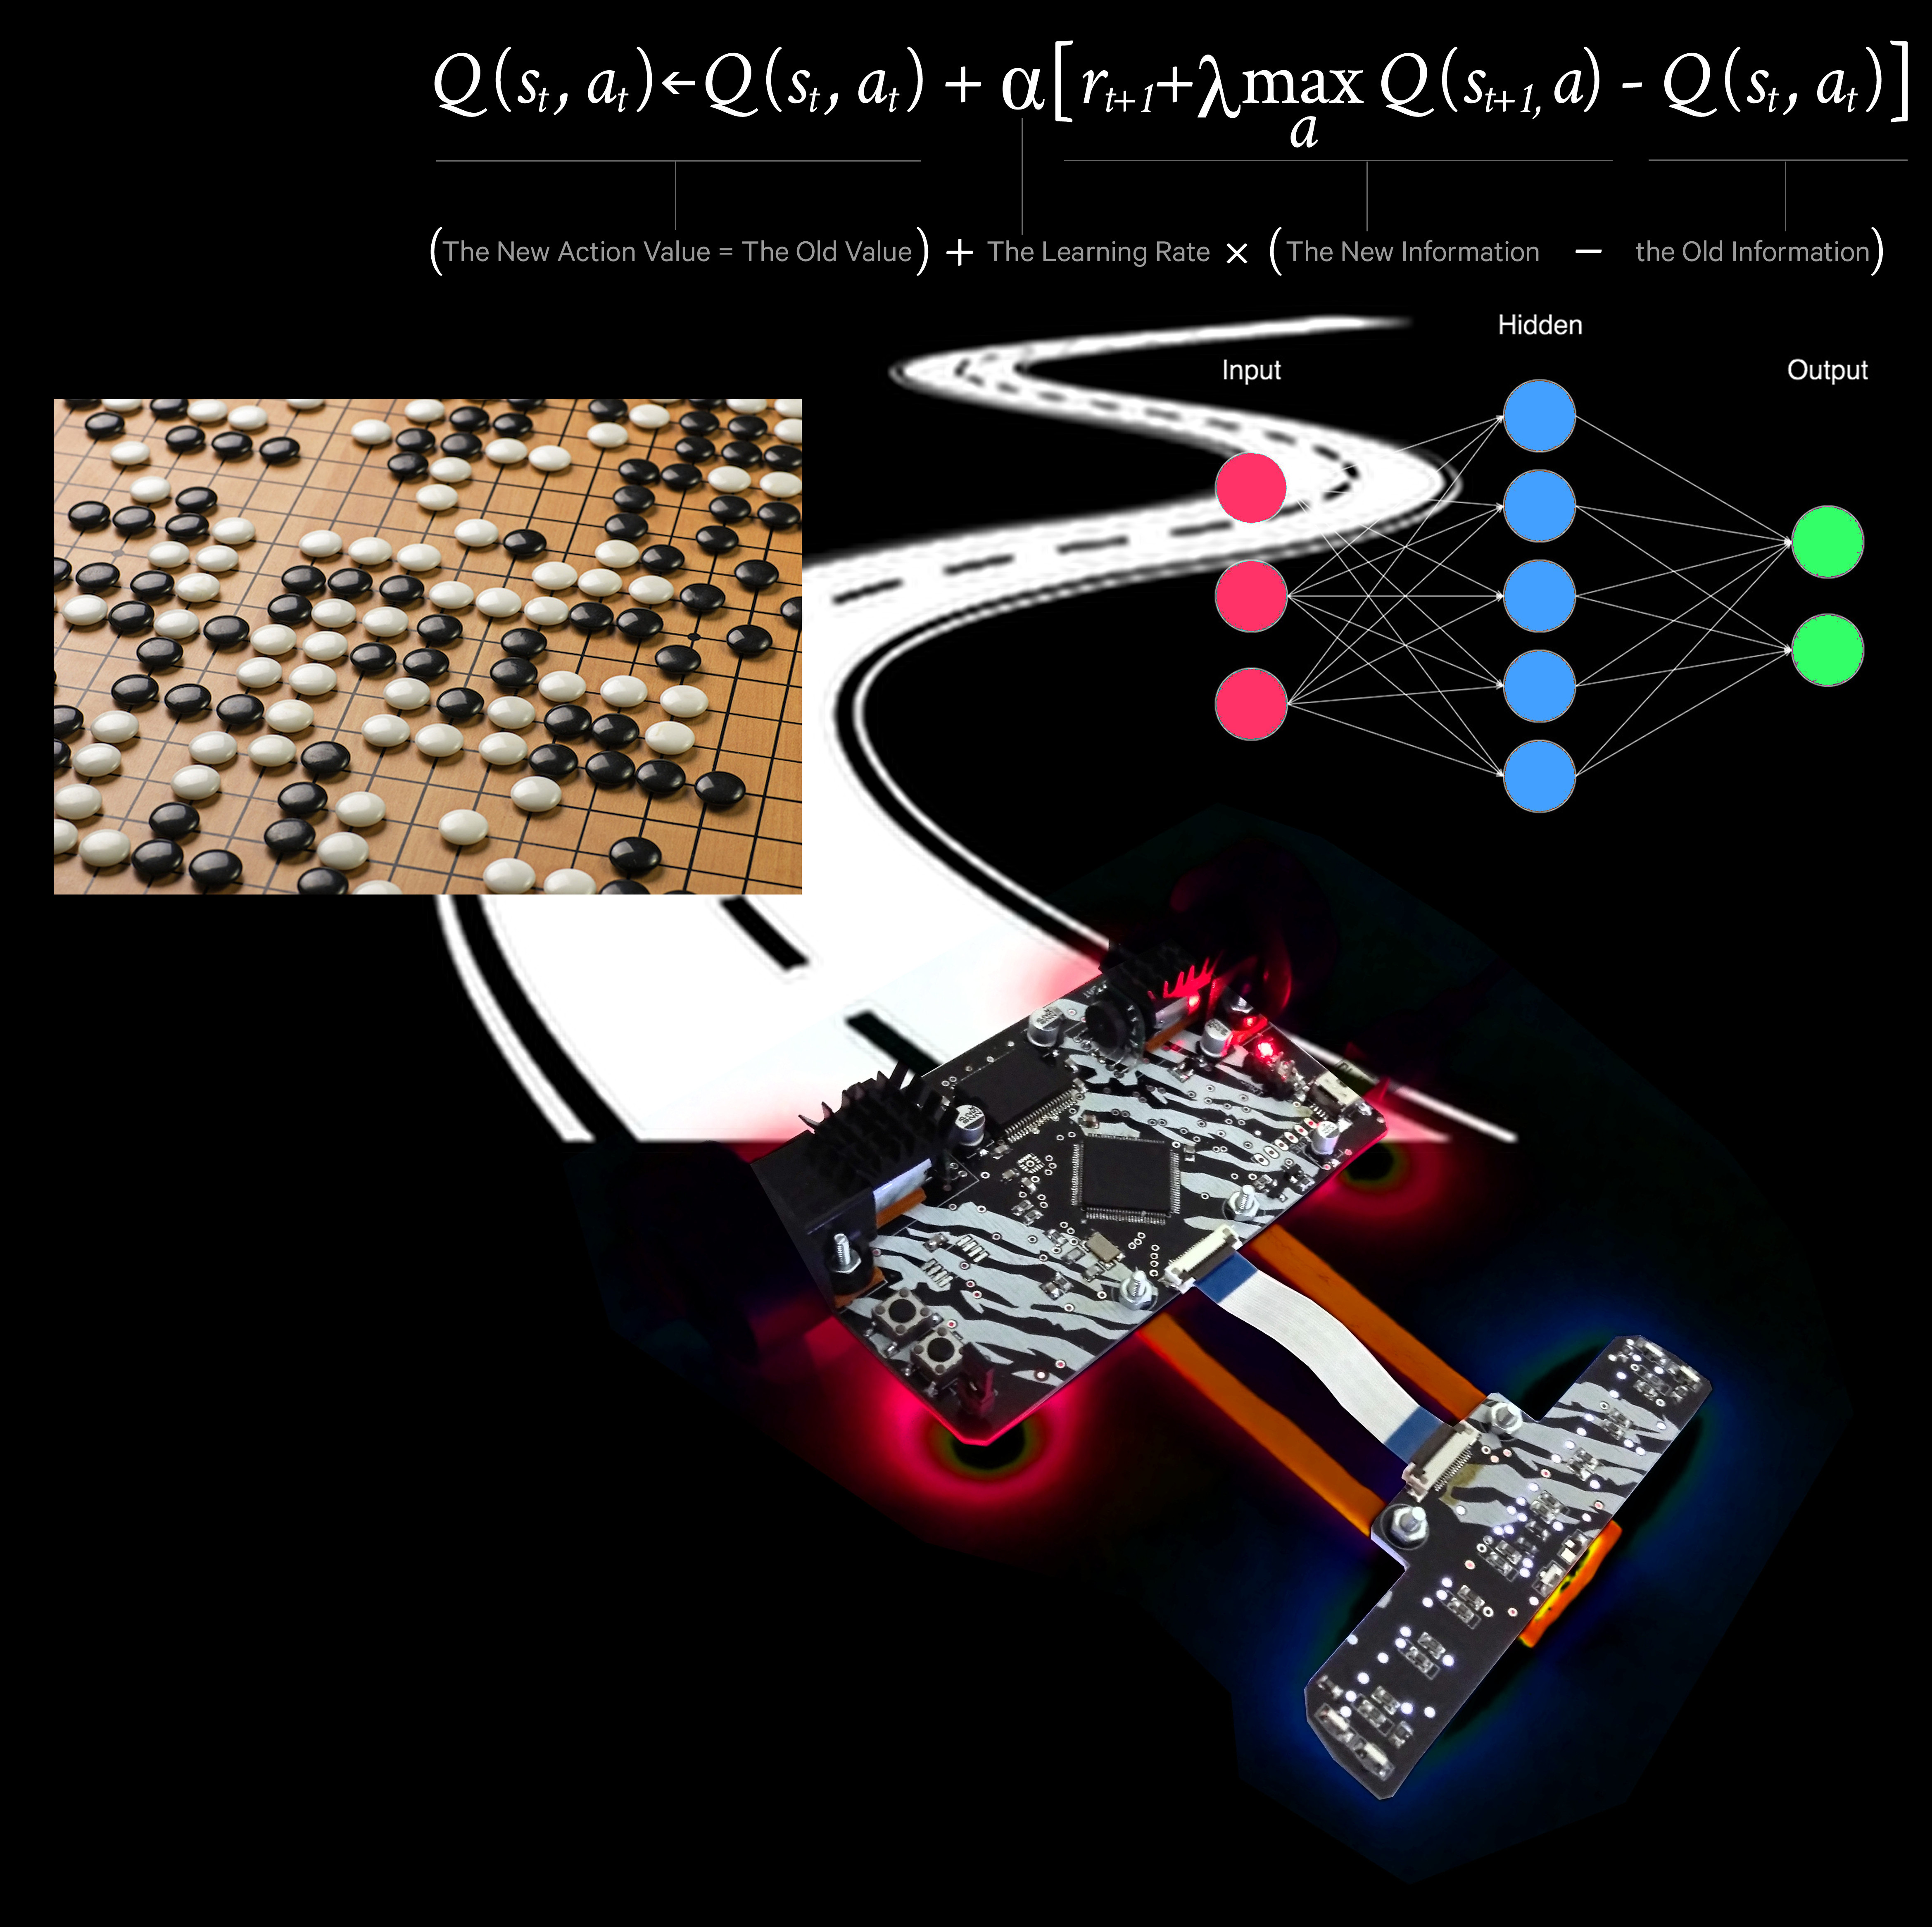
\includegraphics[width=5.05in]{../images/rl_square.jpg}}

        \hfil}\vfil}
    }



    \begin{frame}

    \centering
     \colorbox{black}
     {
        \begin{minipage}{8cm}
           {\LARGE \color{white}deep reinforcement learning 1} \\
           {\Large \color{white}- deep Q networks} \\
           {\Large \color{white}- deep deterministic policy gradient} \\
           {\LARGE \color{white} Michal CHOVANEC} \\
       \end{minipage}
     }

    \end{frame}
}

\begin{frame}{\bf reinforcement learning}

  \begin{columns}

    \begin{column}{0.5\textwidth}
      {\centering 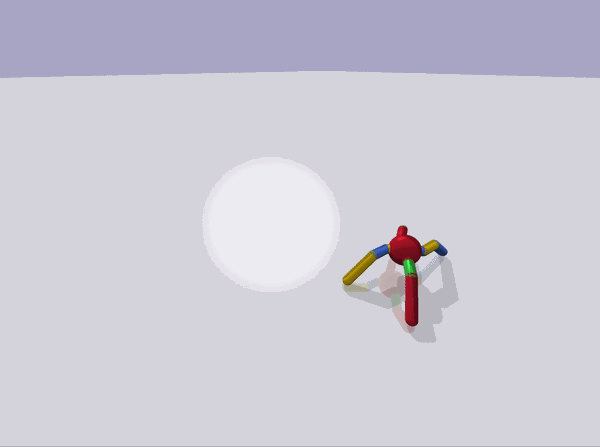
\includegraphics[scale=0.2]{../images/ant.png}}
      {\centering 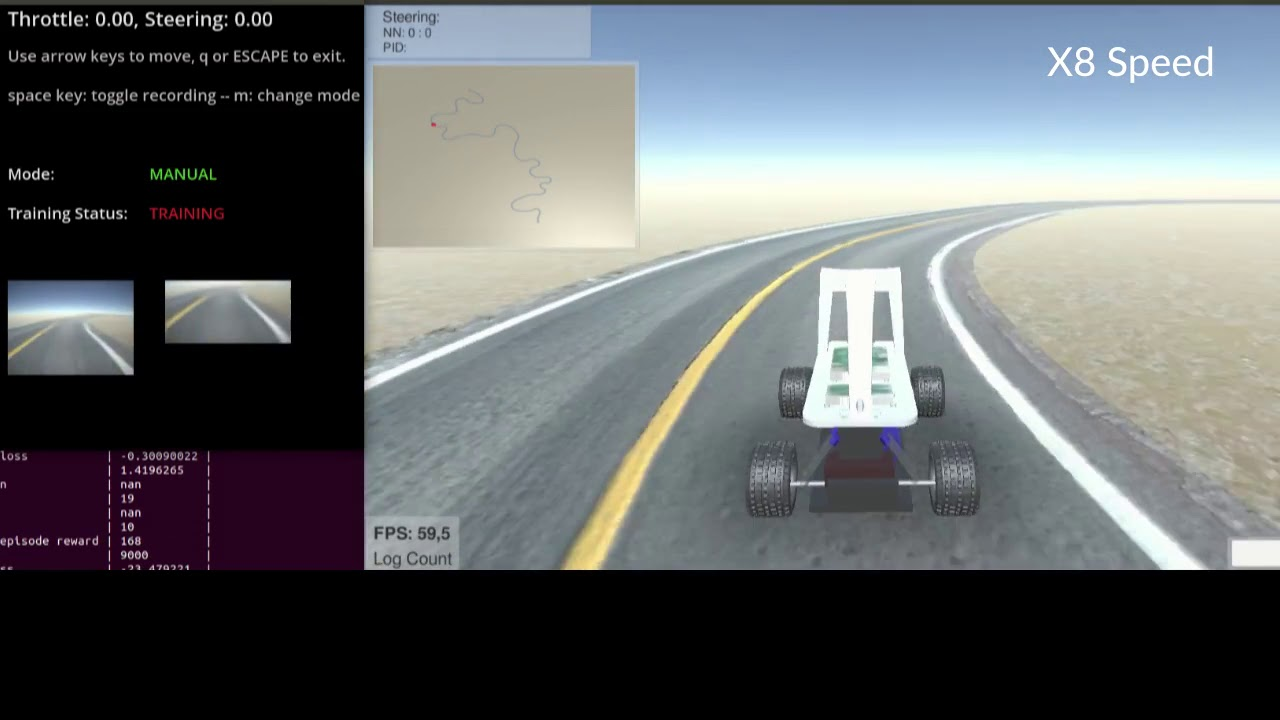
\includegraphics[scale=0.1]{../images/sac_car.jpg}}
    \end{column}

    \begin{column}{0.5\textwidth}
      {\centering 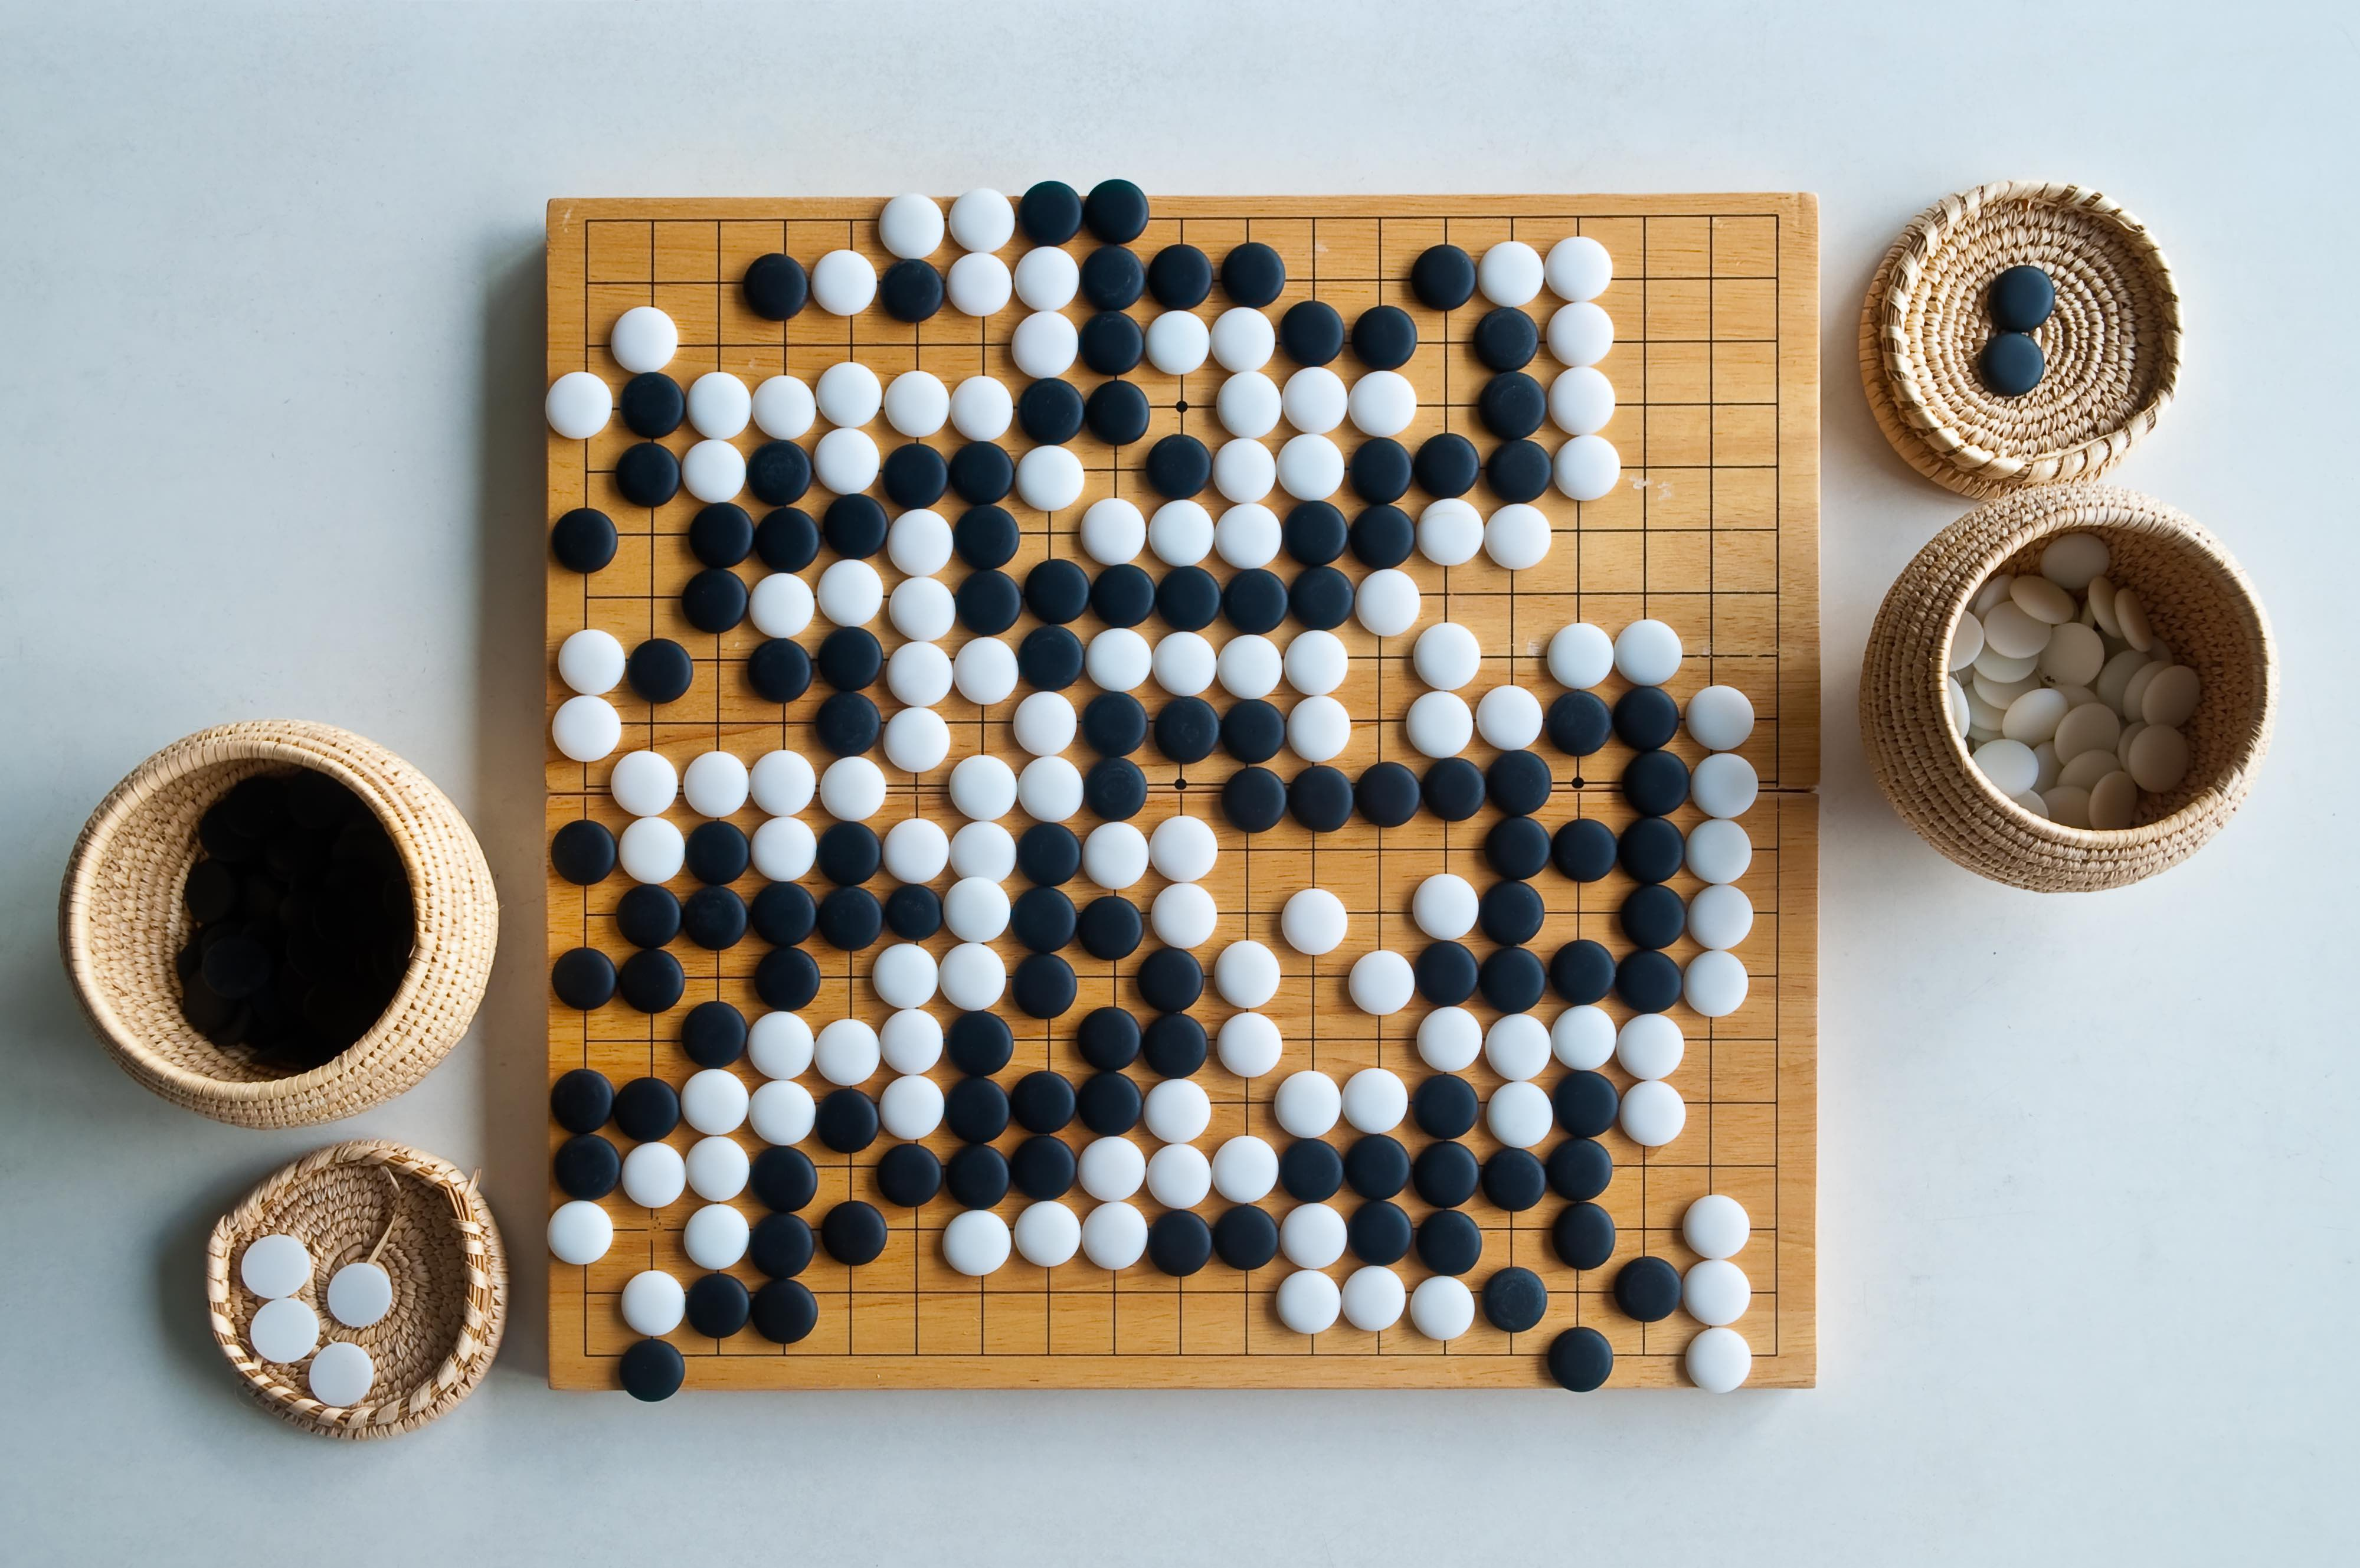
\includegraphics[scale=0.03]{../images/go.jpg}}
      {\centering 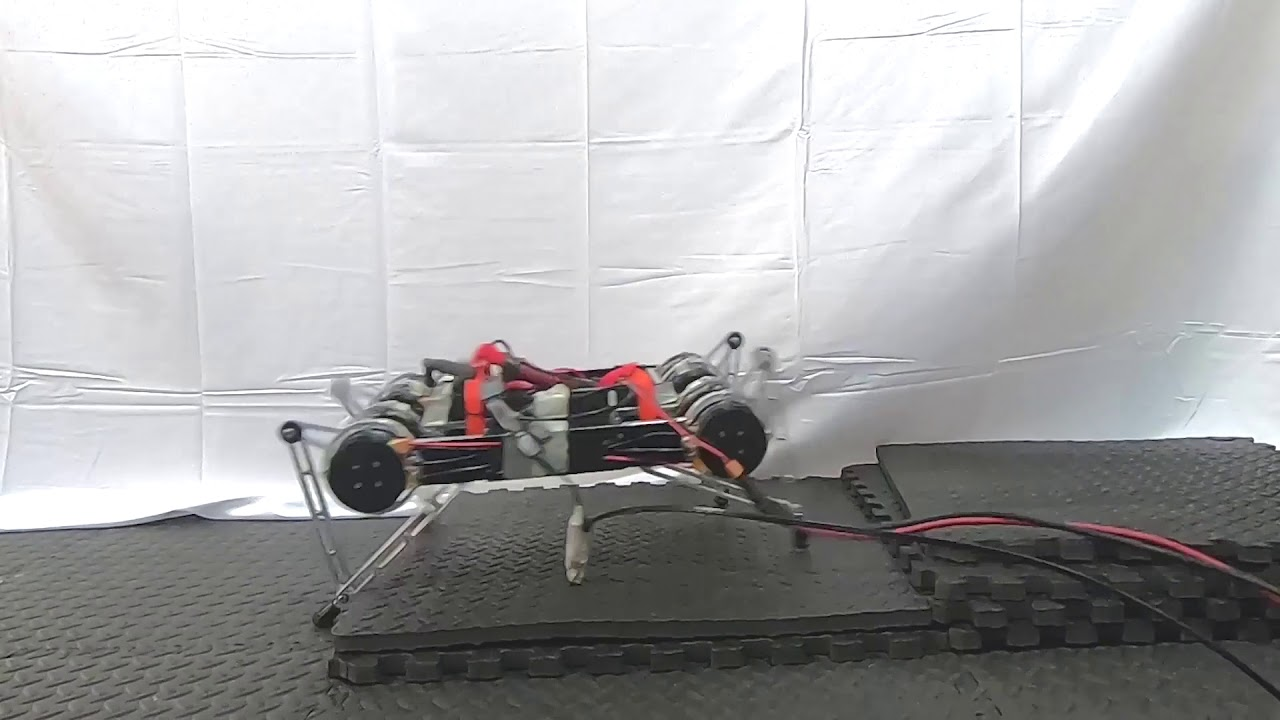
\includegraphics[scale=0.1]{../images/sac_minitaur.jpg}}
    \end{column}


  \end{columns}

\end{frame}


\begin{frame}{\bf reinforcement learning}

  {\bf learning from punishments and rewards \\}
  {\centering 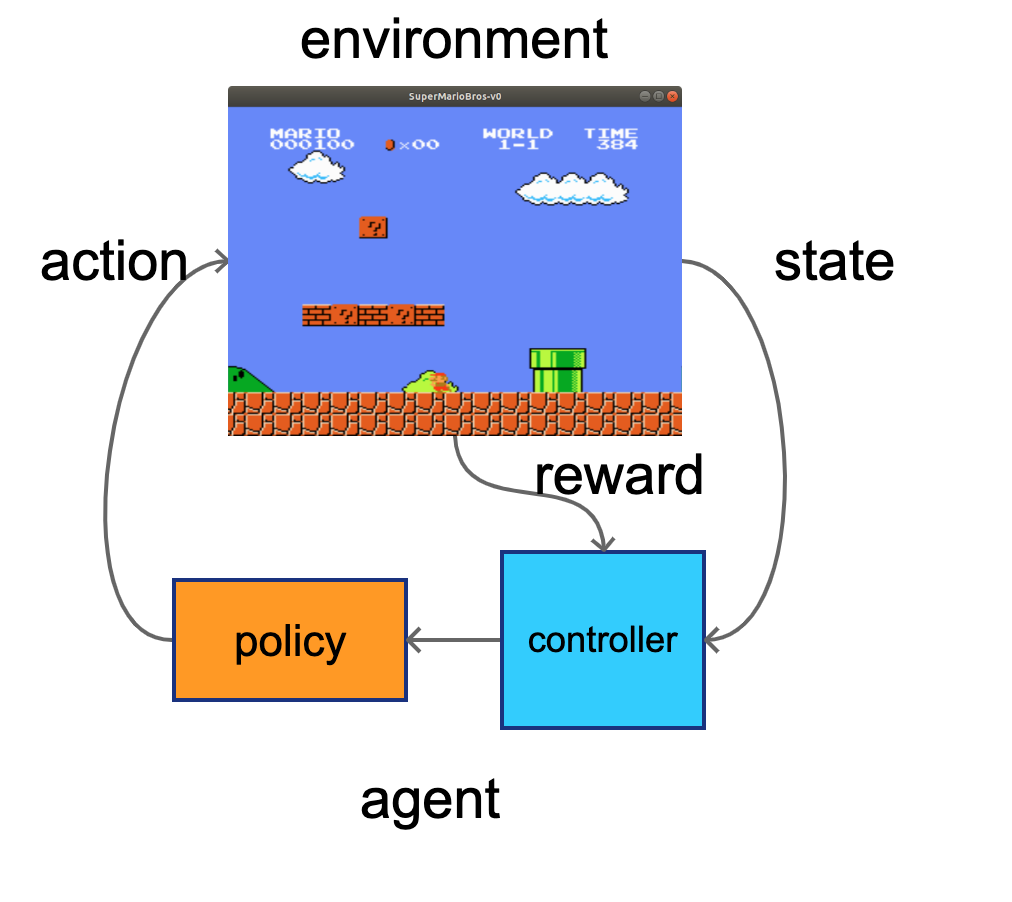
\includegraphics[scale=0.2]{../diagrams/basic/reinforcementlearning.png}}

\end{frame}


\begin{frame}{\bf reinforcement learning}

  \begin{columns}

    \begin{column}{0.5\textwidth}
      {\centering 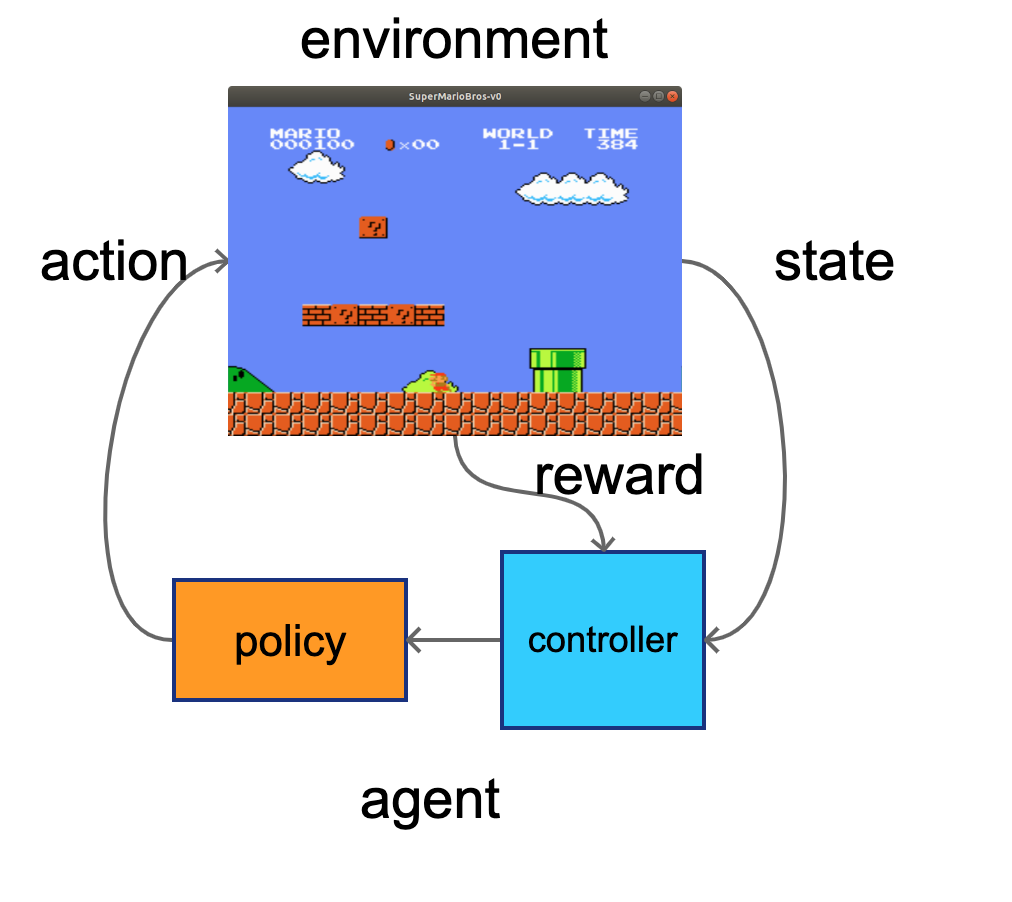
\includegraphics[scale=0.15]{../diagrams/basic/reinforcementlearning.png}}
    \end{column}

    \begin{column}{0.5\textwidth}
      \begin{itemize}
        \item obtain state
        \item select action
        \item exectute action
        \item learn from experiences
      \end{itemize}
    \end{column}

  \end{columns}

\end{frame}


\begin{frame}{\bf action space}

  \begin{itemize}
    \item discrete action space \\
      - keys, keypad
    \item continuous action space \\
      - motors, PWMs, steering, force controll
  \end{itemize}

  {\centering 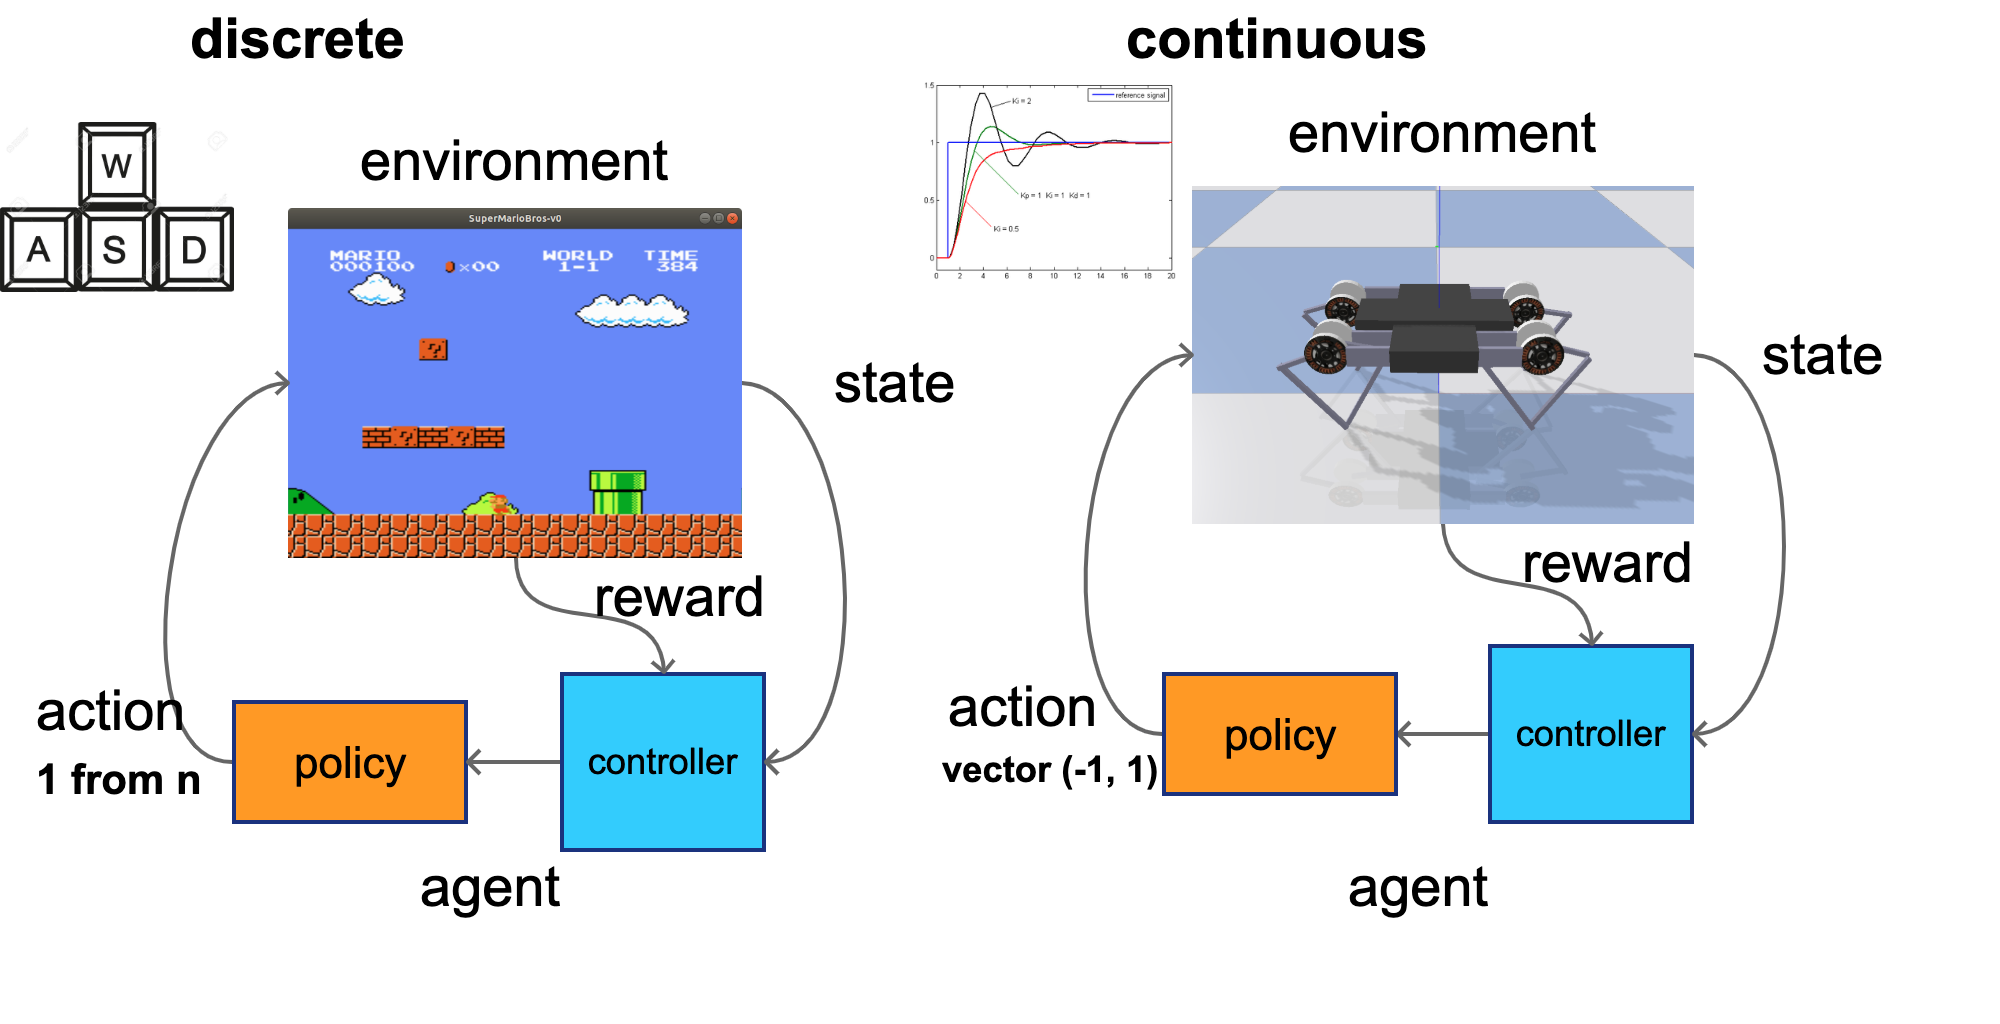
\includegraphics[scale=0.15]{../diagrams/basic/actionspace.png}}

\end{frame}


\begin{frame}{\bf deep Q learning}

  {\centering 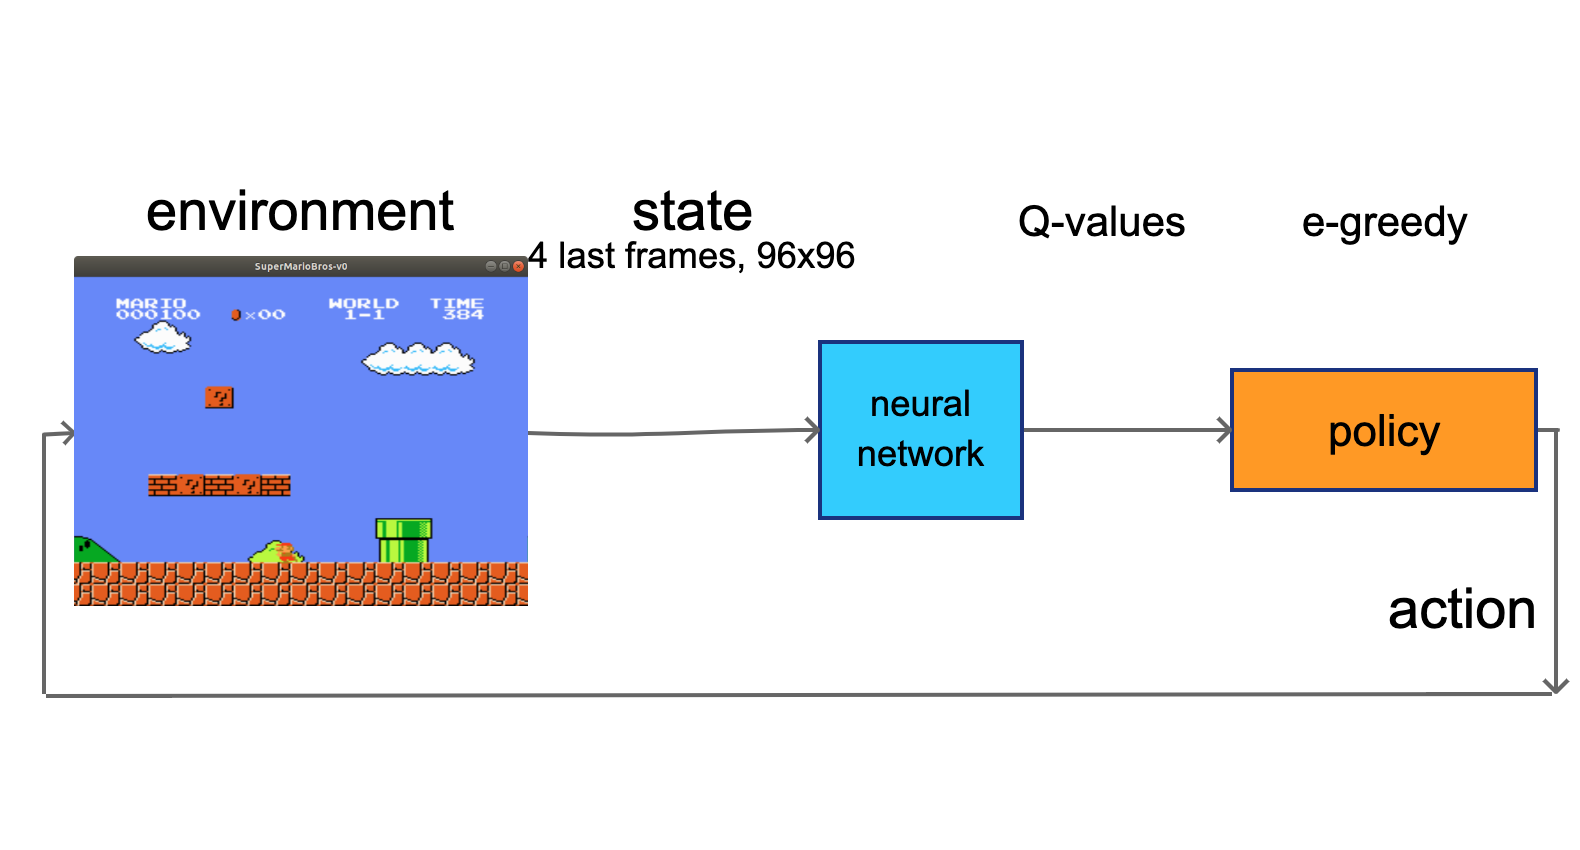
\includegraphics[scale=0.15]{../diagrams/basic/deepqnetwork.png}}

  \begin{enumerate}
    \item play games
    \item store transitions into buffer \\
      - state, action, reward, done
    \item learn from buffer
  \end{enumerate}
\end{frame}


\begin{frame}{\bf deep Q learning}

  {\centering 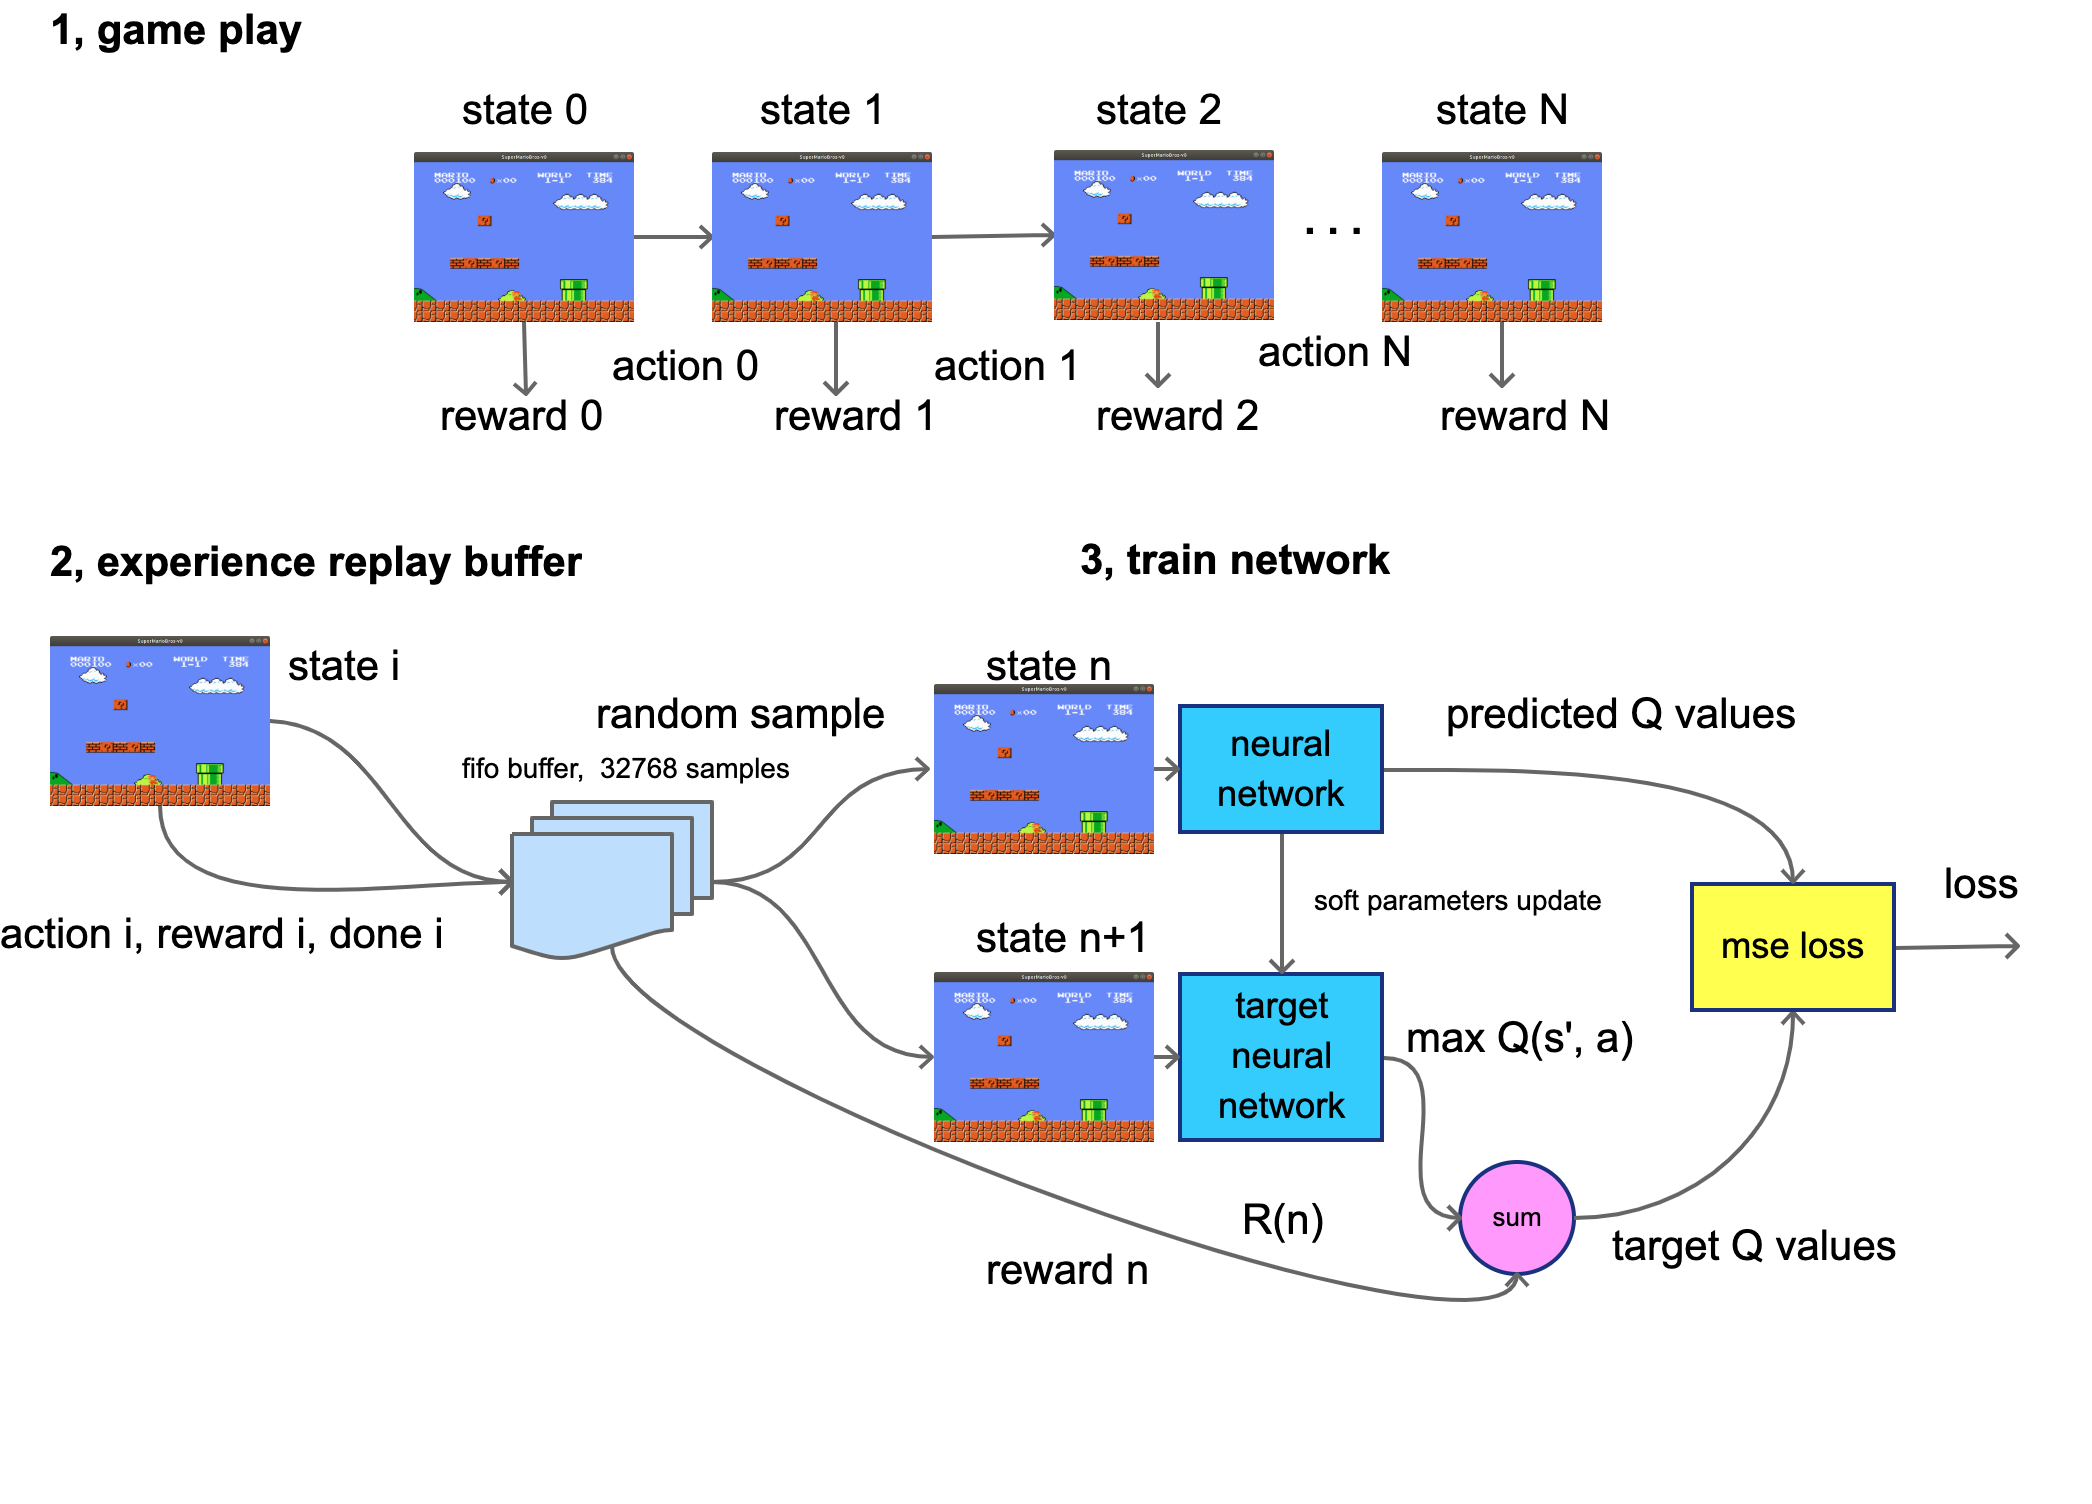
\includegraphics[scale=0.15]{../diagrams/basic/deepqlearning.png}}

\end{frame}


\begin{frame}{\bf deep Q learning}

  {\centering 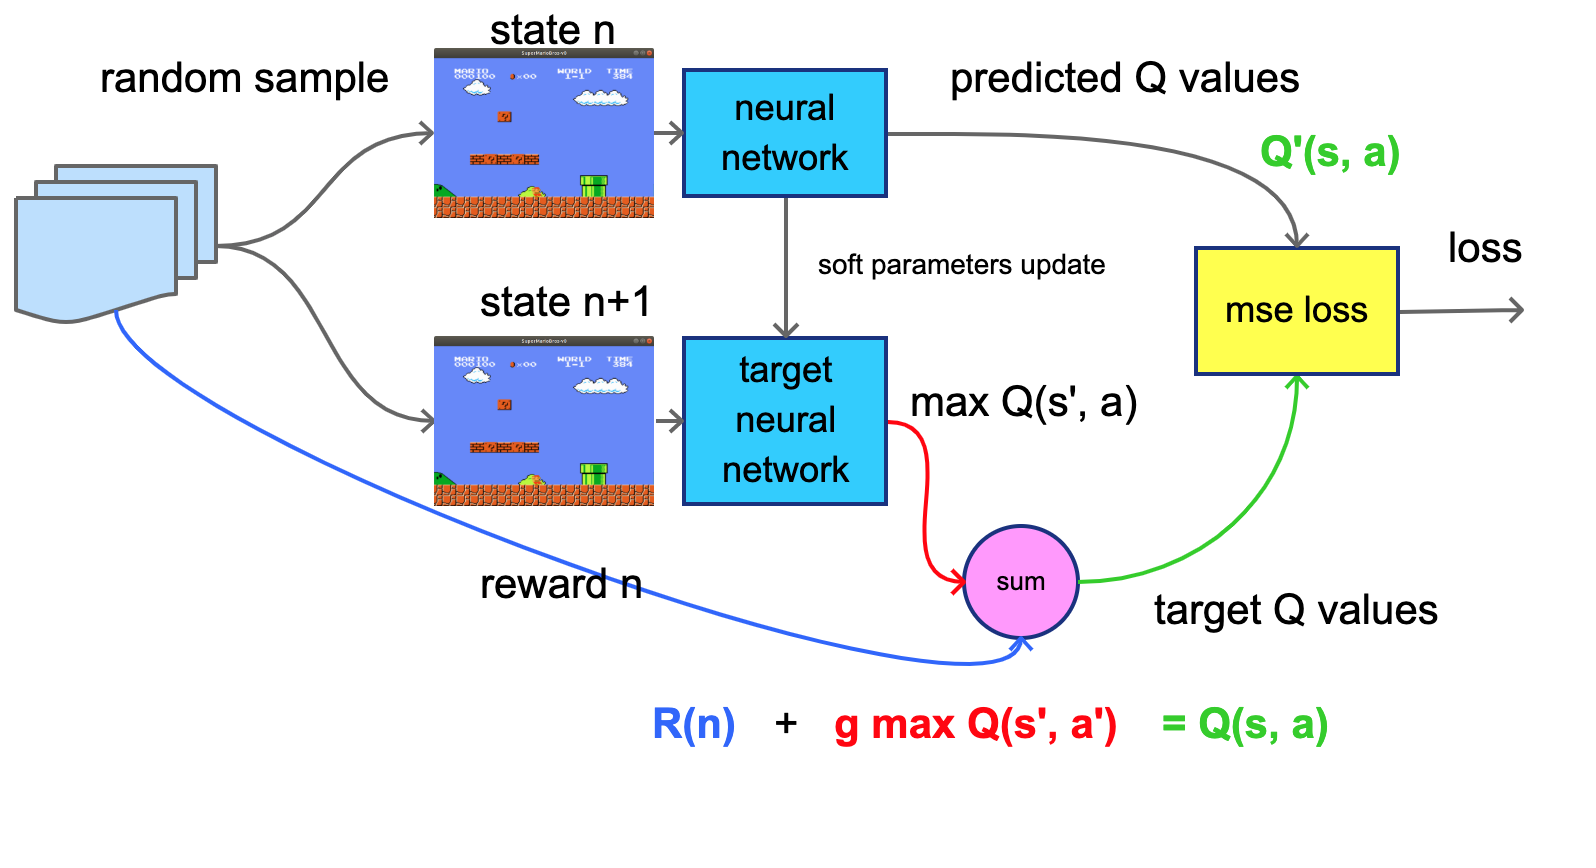
\includegraphics[scale=0.15]{../diagrams/basic/deepqlearningdetail.png}}

  \begin{align*}
    Q(s, a; \theta) = \underset{\textcolor{cyan}{reward}}{R} + \underset{\textcolor{OrangeRed}{discounted\ future\ reward}}{\gamma \max \limits_{a'} Q(s', a'; \theta^-)}
  \end{align*}

  \begin{align*}
    \mathcal{L(\theta)} = \left( R + \gamma \max \limits_{a'} Q(s', a'; \theta^-) - Q(s, a; \theta)  \right)^2
  \end{align*}
\end{frame}


\begin{frame}{\bf model architecture}

  {\centering 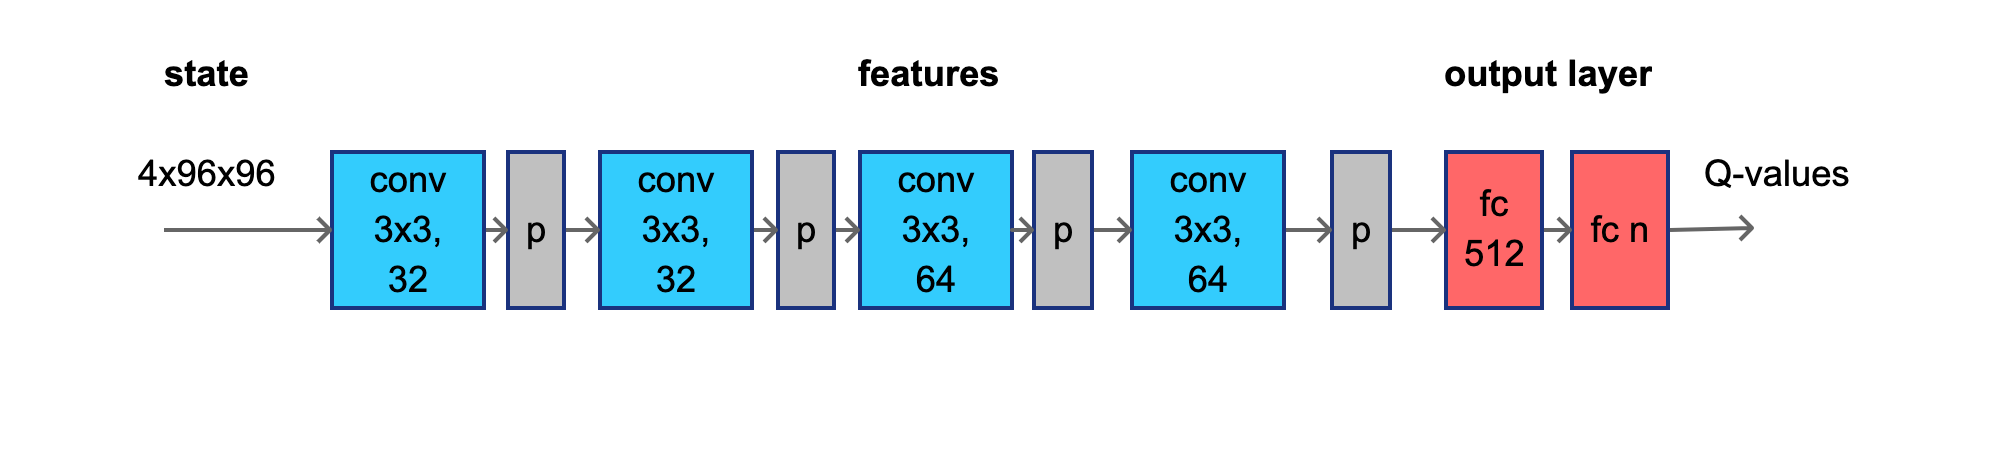
\includegraphics[scale=0.15]{../diagrams/architectures/dqnbasic.png}}

  \begin{itemize}
    \item input 96x96 grayscale, 4 stacked frames
    \item 3x3 convs + pooling
    \item two fully connected layers
    \item small learning rate $\eta = 0.0001$, batch size = 32
    \item $\gamma = 0.99$
    \item exploration $\epsilon$-greedy, 1M samples linear decay from 1 to 0.05
    \item total training 10M samples
  \end{itemize}
 
\end{frame}


\begin{frame}{\bf dueling DQN, model architecture}

  {\centering 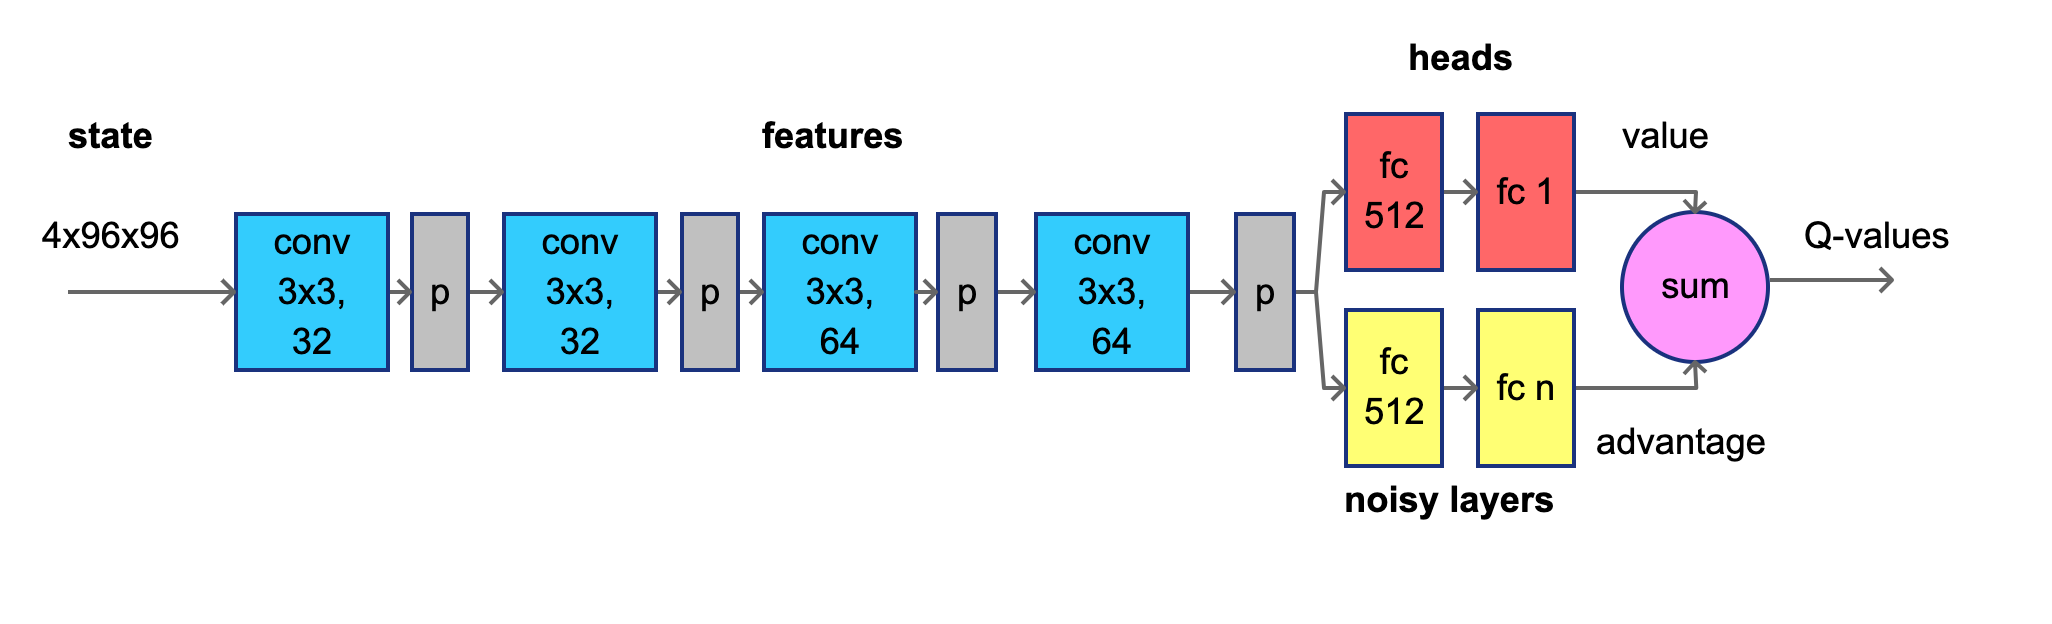
\includegraphics[scale=0.15]{../diagrams/architectures/duelingdqn.png}}

  \begin{align*}
    Q(s, a) &= V(s) + A(s, a) \\
    Q(s, a) &= V(s) + A(s, a) - \frac{1}{|\mathcal{A}|}\sum_{a' \in \mathcal{A}}A(s, a')
  \end{align*}

  \centering{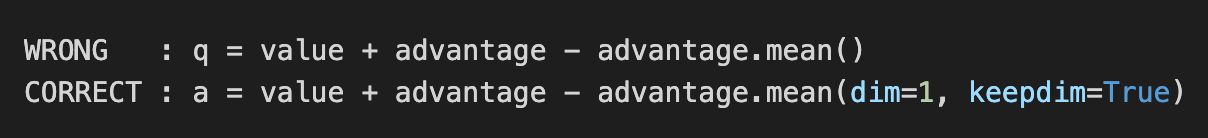
\includegraphics[scale=0.5]{../images/dueling_dqn_code.png}}

\end{frame}


\begin{frame}{\bf noisy layers for exploration}


\centering{\bf {action space noise}}

\centering{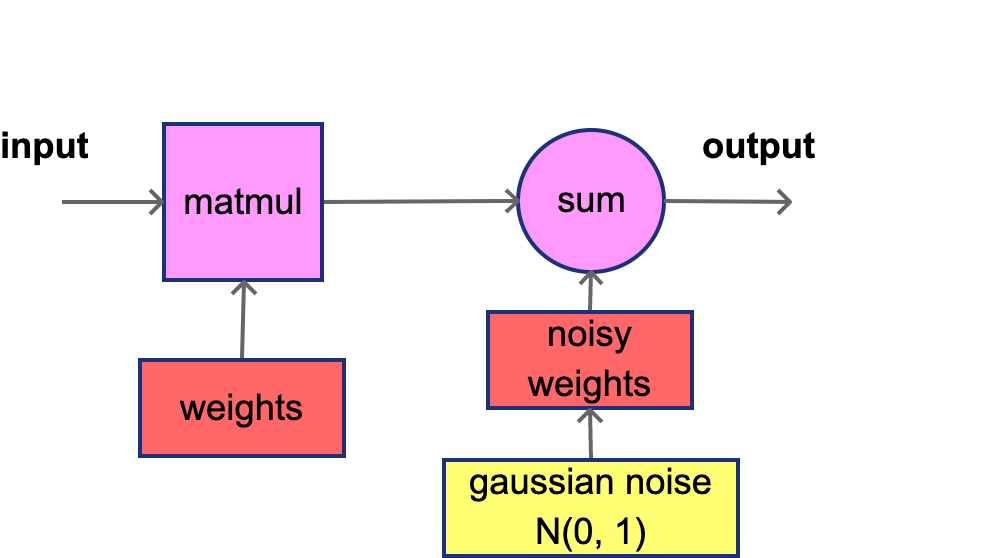
\includegraphics[scale=0.15]{../diagrams/architectures/noisylayerbasic.png}}

\centering{\bf {parameter space noise}}

\centering{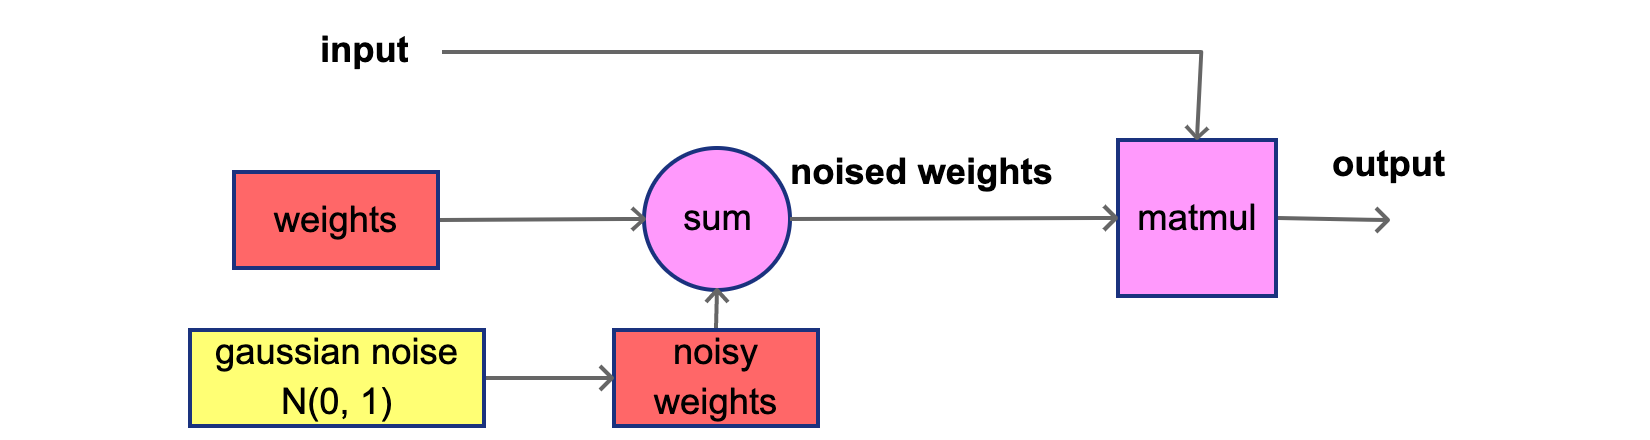
\includegraphics[scale=0.15]{../diagrams/architectures/noisylayerparameter.png}}

\end{frame}



\begin{frame}{\bf books to read}

\begin{itemize}
  \item Maxim Lapan, 2020, Deep Reinforcement Learning Hands-On second edition
  \item Maxim Lapan, 2018, Deep Reinforcement Learning Hands-On
  \item Praveen Palanisamy, 2018, Hands-On Intelligent Agents with OpenAI Gym
  \item Andrea Lonza, 2019, Reinforcement Learning Algorithms with Python
  \item Rajalingappaa Shanmugamani, 2019, Python Reinforcement Learning
  \item Micheal Lanham, 2019, Hands-On Deep Learning for Games
\end{itemize}


\end{frame}

\begin{frame}{\bf Q\&A}

{\centering 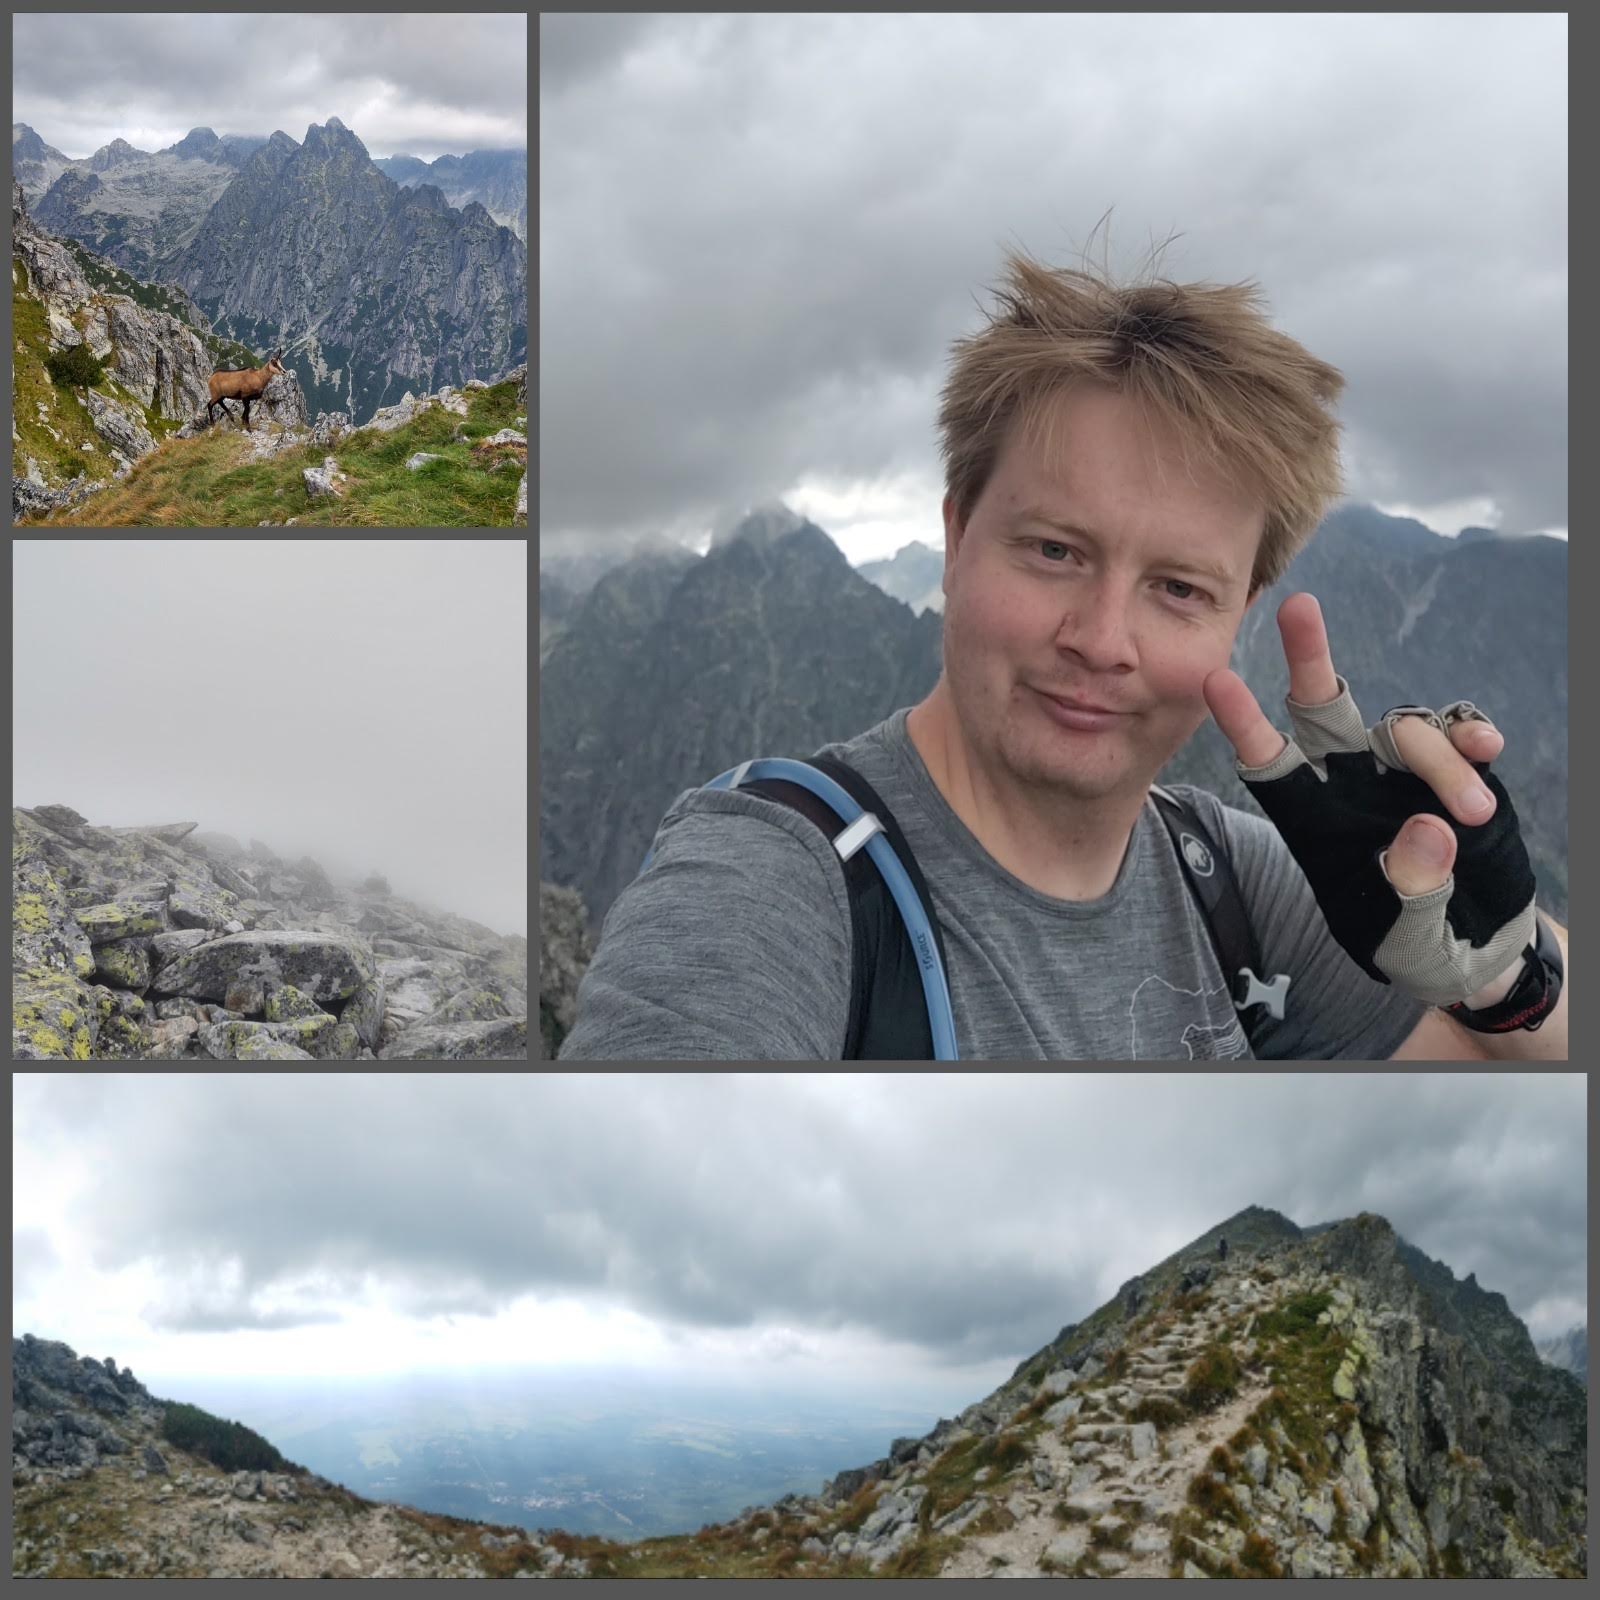
\includegraphics[scale=0.1]{../images/me.jpg}}

\url{michal.nand@gmail.com}

\url{https://github.com/michalnand/imagination_reinforcement_learning}

 
\end{frame}


\end{document}
